%# -*- coding: utf-8-unix -*-
%%==================================================
%% chapter02.tex for SJTU Master Thesis
%% based on CASthesis
%% modified by wei.jianwen@gmail.com
%% Encoding: UTF-8
%%==================================================

\chapter{建模与分析}
\label{chap:example}
我们首先定义锁K的吞吐率为单位时间内K在相关线程间的的平均传递次数,定义单个线程T的吞吐率为单位时间内K在T上平均传递次数。此外,本文中锁K的长期公平性指的是长远来看,各个线程的吞吐率之间的差异程度,可以用变异系数来衡量,变异系数越小,长期公平性越好。线程放置策略决定了线程在NUMA节点之间的分布,进而影响锁在NUMA架构机器上的吞吐率。而对于层级锁来说,由于其本地偏好的锁传递规则的影响,线程放置策略还会影响其长期公平性。本章以两层的MCS锁即cstmcs锁为例,首先通过实验验证紧凑策略和平均策略在对基于队列的层级锁的吞吐率和长期公平性方面的表现,然后建模分析线程放置策略影响吞吐率和长期公平性的根本因素,进而得出线程放置策略优化应遵循的原则和面临的挑战。

\section{实验验证}
我们的实验跑在Intel Xeon E5上,该机器由四个NUMA节点组成,每个节点上包含八个计算核心。实验的benchmark取自libslock中的stress\_one,实验中用到的锁是cstmcs锁,该锁是一个两层的MCS锁,包括一个全局MCS锁和每个节点上的本地MCS锁。实验中stress\_one被配置为使用12个线程,每个线程重复以下操作:拿锁,写一定大小的缓存,放锁,暂停一段时间。该实验中我们用暂停时间的长短来控制锁的竞争强度的大小,暂停时间越长,锁的竞争越激烈,实验中用到了两个暂停
时\begin{table}[!hpb]
  \centering
  \bicaption[指向一个表格的表目录索引]
    {总吞吐率(acquisitions/s)}
    {Aggregate Throughput}
  \label{tab:aggregate}
  \begin{tabular}{@{}llr@{}} \toprule
    暂停时长 & 紧凑放置 & 平均放置\\ \midrule
    5000 cycles & 4574093 & 3101512 \\
    500  cycles & 4401877 & 4273903\\
  \end{tabular}
\end{table}
间:500时钟周期和5000时钟周期。图\ref{Fig:compact}和图\ref{Fig:even}分别展示了该实验在紧凑和平均(AHMCS中将平均放置到所有节点上,而本实验中也是平均放置,但为了获得更高吞吐率,我们是只使用了两个节点)两种放置策略下单个线程的吞吐率,其中在平均放置策略中我们只是用了4个NUMA节点中的两个节点。上述两张实验图中每个长条代表单个线程的吞吐率,而不同颜色表示不同的竞争强度。表\ref{tab:aggregate}和表\ref{tab:CV}分别显示了不同配置下总的吞吐率及变异系数。

\begin{table}[!hpb]
  \centering
  \bicaption[指向一个表格的表目录索引]
    {变异系数}
    {Coefficient of Variance}
  \label{tab:CV}
  \begin{tabular}{@{}llr@{}} \toprule
    暂停时长 & 紧凑放置 & 平均放置\\ \midrule
    5000 cycles & 64.174778\% & 1.939154\%\\
    500  cycles & 35.315475\% & 0.036318\%\\
  \end{tabular}
\end{table}

从表\ref{tab:aggregate}中可以看出,两种竞争强度下的最高吞吐率比较接近,即增加单个线程的锁请求频率并未增加总的吞吐率,所以上述两种竞争强度下cstmcs锁都已经达到了饱和。在锁达到饱和并且关键区域执行时间不变的情况下,影响总的吞吐率的最主要的因素将是锁传递的平均时延大小,而在NUMA架构下影响锁传递平均时延大小的主要是锁在NUMA节点之间传递的频率。

结合图\ref{Fig:compact}、表\ref{tab:aggregate}和表\ref{tab:CV}可以看出紧凑放置能够尽可能地保证层级锁地高吞吐率,但是总的吞吐率在线程之间地分布是严重不均衡的,同一个NUMA节点上地线程吞吐率基本相同,不同NUMA节点上地线程之间吞吐率差别可以达到十几倍,而且实验中的两种竞争强度下受益的线程集合正好相反。结合图\ref{Fig:even}、表\ref{tab:aggregate}和表\ref{tab:CV}可以看出平均放置能够保证层级锁地长期公平性,单个线程的吞吐率之间没有明显地差异,但是即使在总的竞争已经饱和而且在平均放置的基础上使线程放置地尽可能地紧凑地情况下,如果竞争并不是很高其总的吞吐率相比紧凑放置还是有明显地损失,实验中其严重吞吐率损失多大32.2\%。

\begin{figure}[t]
	\centering
	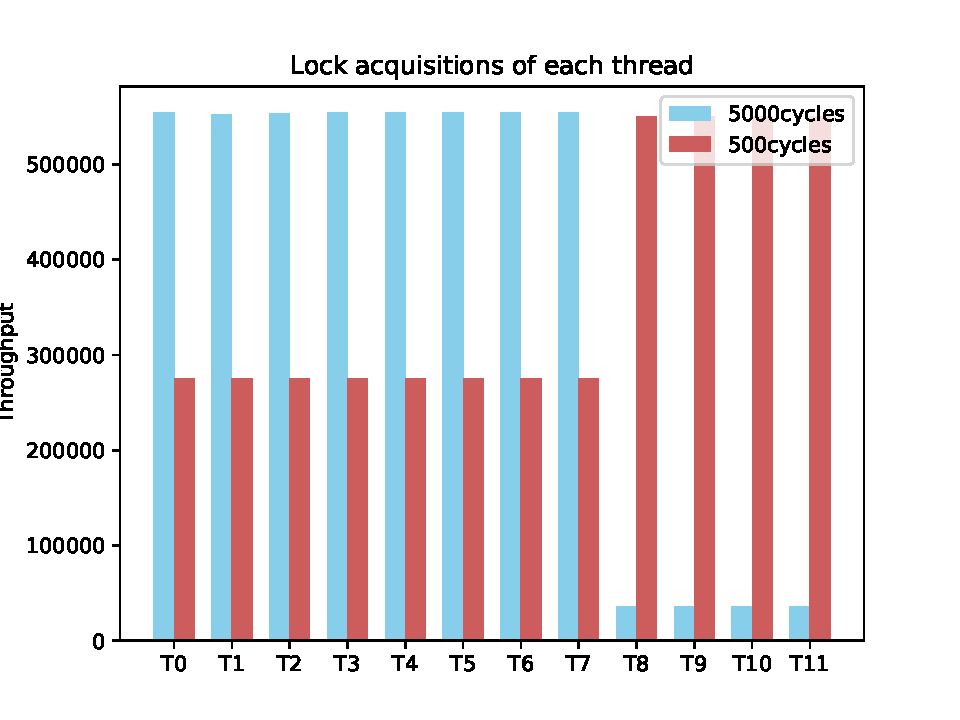
\includegraphics[width=5.6in]{compact.pdf}
	\caption{紧凑放置:单个线程的吞吐率}
	\label{Fig:compact}
\end{figure}

\begin{figure}[t]
	\centering
	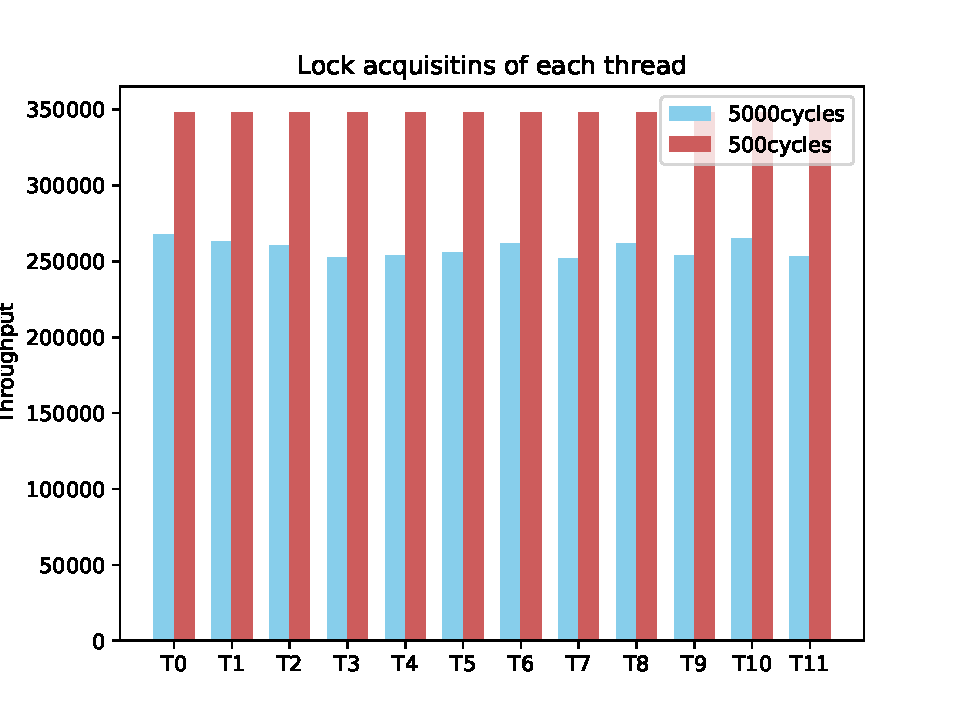
\includegraphics[width=5.6in]{even.pdf}
	\caption{平均放置:单个线程的吞吐率}
	\label{Fig:even}
\end{figure}

\section{单个线程的吞吐率}
以下我们按照层级锁的传递规则建模分析本实验用到的cstmcs锁中单个线程的吞吐率及影响其的主要因素。因为层级锁主要用于竞争线程较多竞争较激烈的场景,所以以下建模分析基于层级锁的竞争较为激烈至少已经饱和的假设。cstmcs锁中用到的全局锁和本地锁都是MCS锁,而MCS锁按照先进先出(FIFO,first in first out)的顺序在线程之间传递,所以我们可以认为全局MCS锁在相关NUMA节点之间按照round-robin的方式传递;对于某个特定节点上的线程来说,当第一个请求者代表该节点拿到全局锁时,对应的本地MCS锁在该节点上运行的所有相关节点之间也按round-Robin的方式传递,直到最后一个请求者释放全局锁(当前节点没有后续请求者)或者某个请求者被强制释放全局锁(当前节点上的传递次数达到threshold),如图\ref{Fig:circulation}所示。为了说明的方便,我们将全局MCS锁在所有相关节点之间传递一次的时间间隔定义为一个循环(circulation),并且以一个循环为单位来评估单个线程的吞吐率。

\begin{figure}[t]
	\centering
	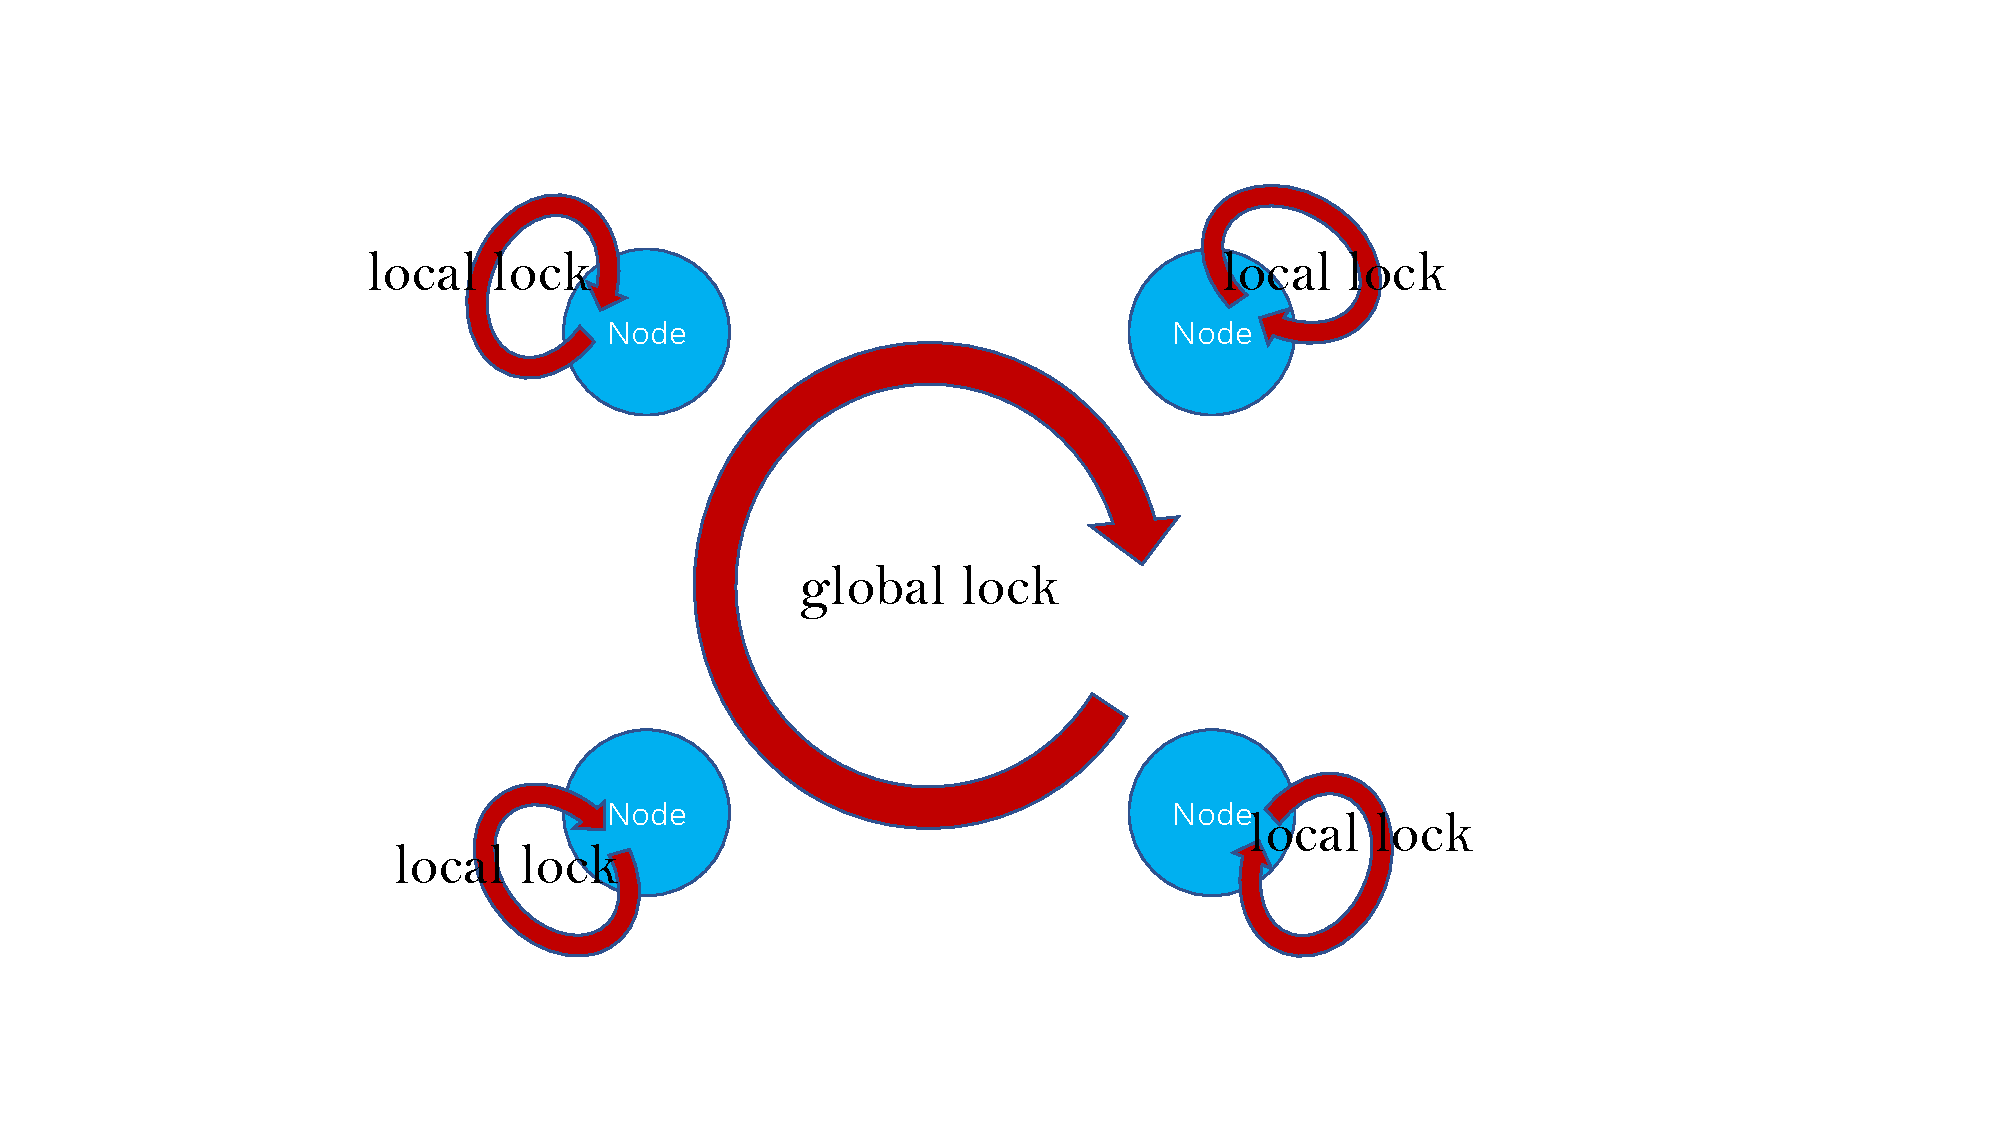
\includegraphics[width=5.6in]{circulation.pdf}
	\caption{cstmcs锁中的一个循环}
	\label{Fig:circulation}
\end{figure}

我们先从简单的情况开始,对于某个特定的线程来说,其在执行或者等待执行关键区域的概率可以表述为:
\begin{equation}\label{Eq:pro}
     P_{cs} = CS / (NCS + CS)
\end{equation}
其中CS和NCS分别代表关键区域和非关键区域的长度。

假如一个应用程序包含T个请求同一个锁的线程,则其在执行或者等待执行关键区域的线程数的期望值为:
\begin{equation}\label{Eq:expectation}
     E_{cs} = T * P_{cs}
\end{equation}

Ecs由应用中锁的竞争者的数量和单个竞争者请求锁的频率计算而来,可以用来表示和评估应用中的锁的总体竞争强度,Ecs越大意味着锁被请求的越频繁,即锁的竞争竞争越大。我们按照Ecs的值跟1的关系将锁的竞争状态定义为以下三种:
\begin{equation}\label{Eq:state}
Lock\ state =
\begin{cases}
under-saturated &\text{Ecs < 1}\\
exact-saturated &\text{Ecs = 1}\\
over-saturated &\text{Ecs > 1}
\end{cases}
\end{equation}
其中恰好饱和(exact-saturated)是锁的一个特殊状态,如图\ref{Fig:saturation}所示,当锁处于饱和态时,锁被持续持有并且所有线程无需等待就能在请求锁的时候就拿到锁。否则或者锁或者不能被持续持有(欠饱和under-saturated)或者线程请求锁之后需要等待一段时间才能拿到锁(过饱和over-saturated)。

根据层级锁的传递规则,在每一个循环中,当某个NUMA节点上的线程使得该节点上的本地锁恰好饱和或者过饱和时,层级锁就能够在该节点上一致传递直到总的传递次数达到预先设定的限制(threshold)为止;否则该节点上每个线程拿锁一次之后就会因为当前节点上没有后续请求者而被强制放弃全局锁,该节点上锁的总传递次数在一个循环内将只有N,其中N是该节点上运行的线程数。即
\begin{equation}\label{Eq:localtrans}
local\ acqs =
\begin{cases}
N &\text{under-saturated}\\
threshold &\text{otherwise}
\end{cases}
\end{equation}
因为MCS锁是完全公平的,所以我们可以认为该节点上每个线程的拿锁次数相等,即每个线程在一个循环里边的拿锁次数为
\begin{equation}\label{Eq:per}
acqs\_per\_thread =
\begin{cases}
1 &\text{under-saturated}\\
threshold / N &\text{otherwise}
\end{cases}
\end{equation}
一般情况下为了获取更高的吞吐率,threshold通常被设为N的若干倍,所以每个节点上放置的线程能否使该节点上的本地锁饱和对于该节点上的每个线程能否获得高吞吐率至关重要。
\section{长期公平性}
在讨论基于队列的层级锁(如cstmcs)的长期公平性之前,我们定义两个线程之间的关系为对称(symmetric)如果不管锁的竞争强度如何变化,这两个线程理论上长期的吞吐率差距为0。由MCS锁的先来先服务的特性可知,运行在同一个NUMA节点上的任何两个线程之间是对称的;而对于运行在两个不同节点上的线程来说,由公式\ref{Eq:per}可知只有当这两个节点上运行的线程数量相等时,这两个线程是对称的。另外,很明显对称关系是一种等价关系,因此所有竞争同一个层级锁的线程可以按照其在NUMA节点上的分布来被分为若干等价类。例如,图\ref{Fig:symmetric}中的20个线程可以分为两个等价类,其中节点0上的8个线程和节点3上的8个线程属于同一个等价类,剩下的4个线程属于另一个等价类。

从上述线程之间的对称关系的定义和分析可以容易看出,层级锁对于同一个等价类中的所有线程是长期公平的,所以在不使用其他额外策略的前提下,只有所有线程都在同一个等价类时层级锁才对于所有线程来说都是长期公平的。也就是说只有所以相关节点上放置的线程数相等时,变异系数为0,此时基于队列的层级锁才能保证长期公平性。这是平均放置能够保证长期公平性的原因,也可以解释为什么图\ref{Fig:compact}中紧凑放置不能保证长期公平性,即图\ref{Fig:compact}中的线程属于两个等价类。而紧凑放置两种竞争强度下受益线程集合互补则可以由公式\ref{Eq:per}来解释,当竞争强度较小(暂停时间为5000 cycles)时,前8个线程所在的节点的本地锁处于饱和或者国饱和态而后4个线程所在的节点的本地MCS锁处于欠饱和态,所以前8个线程的吞吐率远大于后四个线程的吞吐率;当竞争强度较大(暂停时间为500 cycles)时,两个节点上的本地MCS锁都处于饱和或者过饱和态,所以对于只运行四个线程的后一个节点上的线程更有利。

\begin{figure}[t]
	\centering
	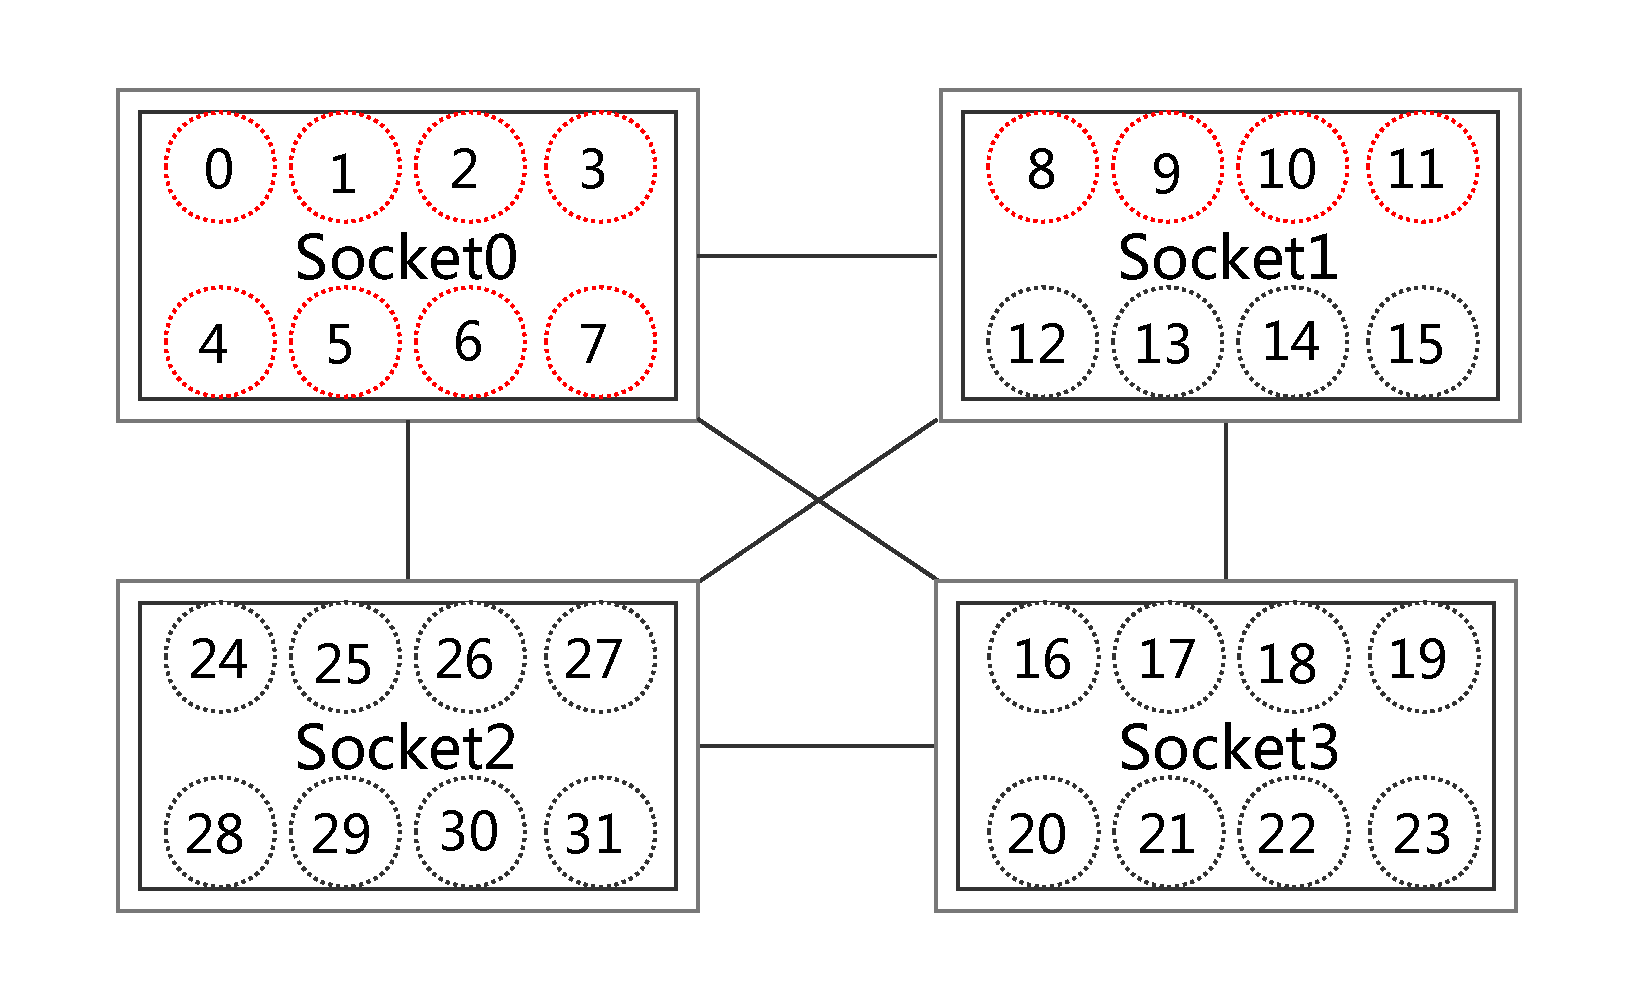
\includegraphics[width=5.6in]{symmetric.pdf}
	\caption{线程等价类}
	\label{Fig:symmetric}
\end{figure}

\section{总吞吐率}
层级锁在竞争强度较大锁达到饱和的情况下其吞吐率大小主要受跨节点的锁传递比例的影响,所以获得更高吞吐率的关键是要减小跨节点锁传递的比例。而在cstmcs中只有全局锁会跨节点传递,所以我们从全局锁的传递角度分析总吞吐率的主要影响因素,我们以一个循环为单位来评估总吞吐率。在每个循环中,全局MCS锁在节点间的传递次数是固定的并且等于相关的节点数目,因此全局锁的跨节点传递比例由每个循环中总的锁传递次数决定。每个循环中每个线程的拿锁次数越多,锁的总传递次数就越多,锁在节点间传递的比例就越小,总吞吐率也就相应越高。根据公式\ref{Eq:per},在每个循环中,单个线程的拿锁次数为1如果其所在的节点的本地MCS锁是欠饱和的,否则其拿锁次数为threshold/N, 一般情况下,threshold会是N的数倍,因此每个本地MCS锁是否达到饱和对于总的吞吐率有很大的影响。而根据公式\ref{Eq:pro}到公式\ref{Eq:state},保证局部MCS锁达到饱和的条件是在相应的节点上放置至少sat个线程,sat是Pcs的倒数
\begin{equation}\label{Eq:sat}
     sat = (NCS + CS) / CS
\end{equation}
这儿sat正是饱和点的大小,如图\ref{Fig:saturation}所示。

在上节的实验中,两种竞争强度下,紧凑放置至少能保证一个节点上的本地锁处于饱和或者过饱和态所以能够保证高吞吐率;而平均放置在竞争强度大(暂停时间500 cycles)时能获得与紧凑放置差不多的吞吐率而在竞争强度较小(暂停时间5000 cycles)是相比紧凑放置吞吐率严重下降的主要原因是,竞争强度高时对应饱和点小,两个节点上的本地锁都能饱和,而竞争强度小时对应饱和点大,两个节点上的本地锁都不能饱和,而上述实验中平均放置在每个节点上的线程数正好处于这两个饱和点之间。

\begin{figure}[t]
	\centering
	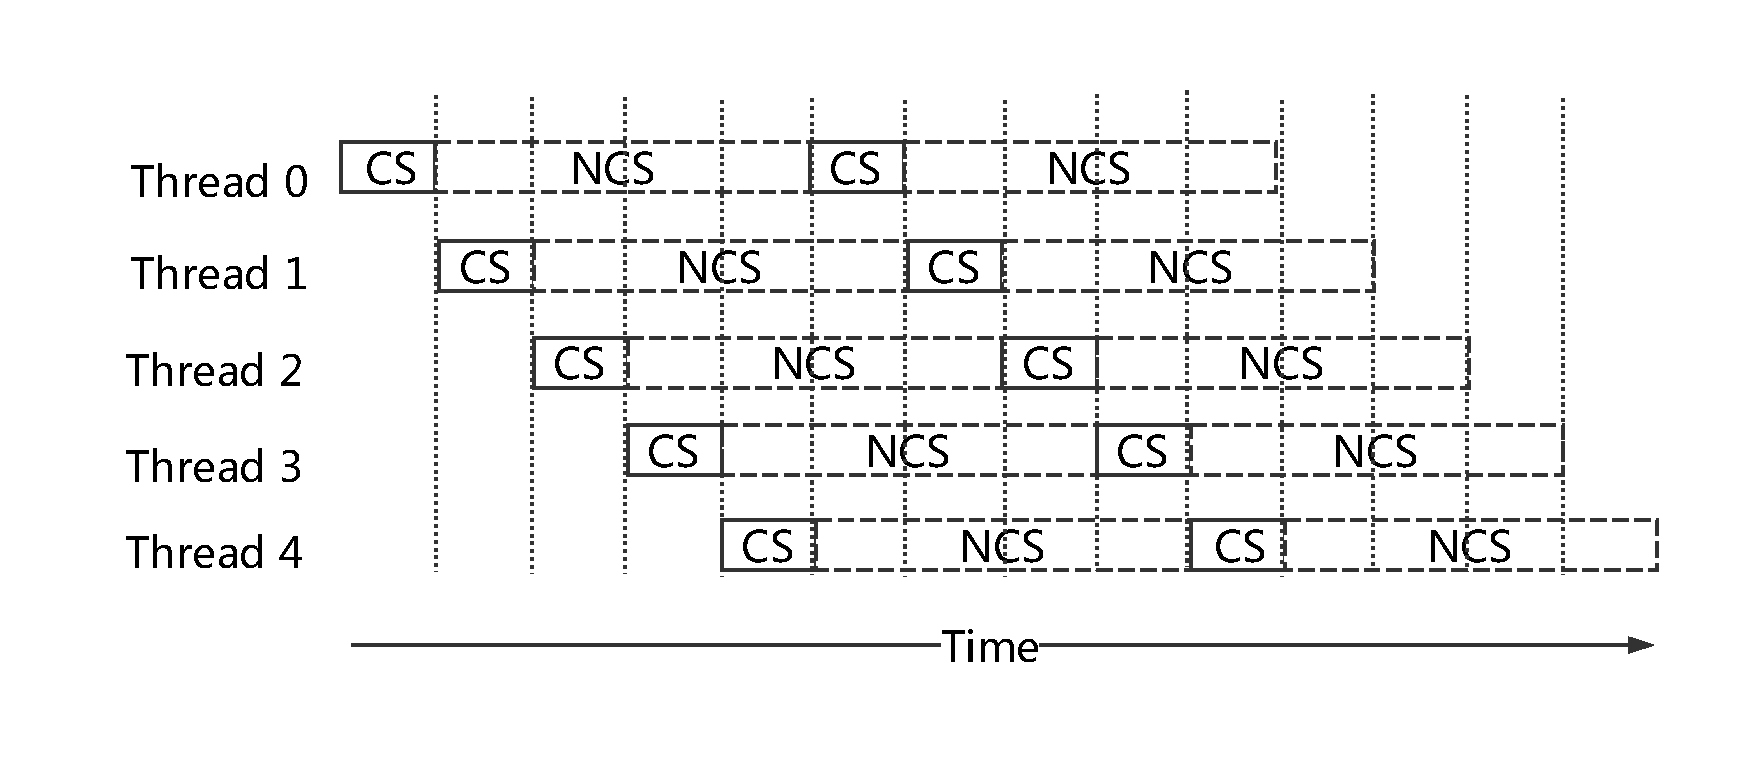
\includegraphics[width=5.6in]{saturation.pdf}
	\caption{饱和点,该图示中饱和点为5}
	\label{Fig:saturation}
\end{figure}

\section{结论与挑战}
通过上述建模和分析我们可以看出,基于队列的层级锁的吞吐率主要与每个节点上的本地锁是否饱和有关,而其长期公平性主要由各个节点上放置的线程数是否相等决定,另外在考虑到自由线程调度存在的缺陷,我们认为从线程放置的角度来优化层级所的吞吐率和长期公平性应该遵循以下原则:
\begin{enumerate}
  \item 保证每个线程运行在一个专用核上;
  \item 使得线程分布在尽可能少的NUMA节点上
  \item 尽可能保证放置在每个相关节点上地线程数达到或超过当前地饱和点;
  \item 尽可能使得每个相关节点上放置地线程数相等;
\end{enumerate}
上述原则中,第一点在避免抢占带来的相关问题;第二点和第三点通过降低锁在节点间地传递比例来提高吞吐率;第四点通过使所有线程变为一个等价类来保证层级所的长期公平性。

紧凑放置遵循了前三点原则,保证了高吞吐率但是存在严重的长期不公平问题;平均放置遵循了第一点和第四点原则,保证了层级所的长期公平性但是存在吞吐率严重下降的问题。现实中很多应用场景比如公有云等对于吞吐率核公平性都有着很高的要求,现有的线程放置策略显然很难满足这些场景的需求。如果能同时满足上述四项原则,则可以同时保证层级所的吞吐率核长期公平性,然而现实中这三点很难同时满足甚至相互冲突,比如本章开始的实验在暂停时间为5000 cycles时不可能同时满足上述四个约束。

在公有云等很多共享资源的场景下,资源的高效利用和资源在用户间的公平分配对于其的成功同等重要;这些应用场景同时也因为价格、时段等因素的影响,资源的需求变化很大,再加上多种应用共享底层硬件资源带来的影响,使得共享资源的竞争很难预测和控制。这些都对共享资源的分配和利用提出了新的挑战,从本章的分析可以看出线程放置对于使用层级锁的应用中的共享资源的利用和其在线程间的分配有很大影响。而显然现有的简单单一的线程放置策略从理论上来说在某些场景下不可能同时保证吞吐率和长期公平性;另外,现实中应用在运行过程中线程数和饱和点这两项决定应用中锁竞争强度大小的因素都可能会随着上层的需求或者下层硬件状态的变化而变化,简单的线程放置策略并不能总是保证吞吐率和长期公平性,这两点也是本文所面临的主要挑战。

显然,简单单一的线程放置策略不能满足应用在各种复杂多变的需求下对层级锁吞吐率和长期公平性的需求,我们需要额外的技术和更复杂更合理更细力度的线程放置来应对这些挑战。

\section{本章小结}
在这一章中,我们首先通过实验展示了现有基于队列的层级锁层级所中线程放置策略在吞吐率和长期公平性方面的表现,然后通过对单个线程的吞吐率进行建模分析除了决定基于队列的层级锁的吞吐率和长期公平性的关键因素,最后在此基础山得出了基于队列的层级锁中线程放置策略应该遵循的基本原则和实现这些基本原则所要面临的挑战,从而为后续说明竞争感知的混合线程放置策略做好了理论基础。